\section{What are fractals?}\label{what-are-fractals}

Fractals are objects with self-similarity, where the smaller fragments are
similar to those on a larger scale. A characteristic feature is to have subtle
details even at very high magnification.\index{fractal}

\subsection{Mandelbrot set}\label{mandelbrot-set}\index{Mandelbrot Set}

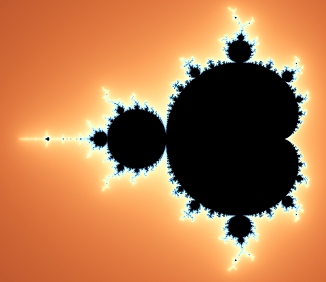
\includegraphics[width=0.5\linewidth]{img/manual/media/mandelbrot_set.png}

This is a typical example of a two-dimensional fractal generated mathematically.
This image is created with a very simple formula, which is calculated in many
iterations:

\[z_{n + 1} = z_{n}^{2} + c\]

\begin{itemize}
	
	
	\item\emph{z} is a complex number (\emph{a} + i\emph{b}), where \emph{i} is
	imaginary number.
	
	\[ i = \sqrt{-1} \]
	
	The number is made of two parts : \emph{a} the real part and i\emph{b} the
	imaginary part.
	
	\item\emph{c} is the coordinates of the image point to be iterated.
\end{itemize}

In 2D, \emph{z} is a vector containing two complex number coordinates , x and y,
( these points represent the pixel location where x represents the real part of
the number {[}a{]} and y represents the imaginary part of the number {[}b{]}).
Because they are complex numbers, they can be positive or negative, but also
there will still be a mathematical solution if a function requires the square
root of a negative number.

Each original point (pixel position) is tested in the formula iteration loop, to
determine if it belongs to the formula specific mathematical fractal set.

The initial value of point \emph{z} is assigned to equal \emph{c}, ($ z_{0} = c
$), this parameter is then used repeatedly in the iteration loop.

\(z_{n + 1} = z_{n}^{2} + c\)

\(z_{n + 2} = z_{n + 1}^{2} + c\)

\(z_{n + 3} = z_{n + 4}^{2} + c\)

etc.

The program has to determine if these series are convergent. To do this
iterations should be repeated infinite number of times. But in this way won't be
possible to get any image. There is used simplification.

Termination conditions are applied to ensure the formula does not iterate to
infinity. The most common conditions used are called \textbf{Bailout} and
\textbf{Maxiter}.

\label{bailout-maxiter}The \textbf{Bailout}\index{termination condition!bailout} condition stops the iteration loop if the formula
transforms (moves) the point further than a set distance away from an
``origin''. This detects if series are convergent (calculated point is outside
the fractal body)

\textbf{Maxiter}\index{termination condition!maxiter} is simply a condition to stop iterating when a maximum numbers
of iterations is reached (just to not do iterations infinite times)

In the Mandelbrot formula, after each iteration, the modulus of a complex number
is calculated; in other words, the length of the vector from the origin
(\emph{x} = 0, \emph{y} = 0) to the current \emph{z} point. This vector length
is often called \emph{r} for it is the radius from the center (origin) to the
current \emph{z} point.

In this example, when the length \emph{r} \textgreater{} 2 (i.e \emph{Bailout} =
2), the termination condition has been met, then the iteration process is
stopped and the resulting image point is marked with a light color. When, after
many repeated iterations, \emph{r} is still less than 2, then it can be
considered for simplicity that such a result will continue indefinitely.
Iterations are therefore interrupted after a certain number of iterations
(Maxiter). This point is marked on the image with black. This results in a
``set'' of points that do not reach bailout termination (black) and the rest of
the points given lighter colors (dependent on a chosen coloring method).

\subsection{3D fractals}\label{d-fractals}

The three dimensional fractal type, the ``Mandelbulb''\index{Mandelbulb} is calculated from a
fairly similar pattern to the Mandelbrot set. The difference is that the vector
\emph{z} contains three complex numbers (\emph{x}, \emph{y}, \emph{z}) or four
dimensions (\emph{x}, \emph{y}, \emph{z}, \emph{w}). As they are part of the
\emph{z} vector, they are denoted as (\emph{z.x}, \emph{z.y}, \emph{z.z}).
Examples being Hypercomplex numbers and quaternions.

They can also be created by modification of quaternions or by a specific
representation of trigonometric vectors. Generally, common maths operators are
used, e.g., addition, multiplication, squaring, and powers), and also
conditional functions ( e.g., \textbf{if} \emph{z.x} \textgreater{} \emph{z.y},
\textbf{then} \emph{z.x} = \emph{something}).

Some other types of 3D fractal objects are based on iterative algorithms (IFS -
Iterated Function Systems\index{IFS}). An example would be the famous Menger Sponge\index{Menger Sponge}.
\nopagebreak

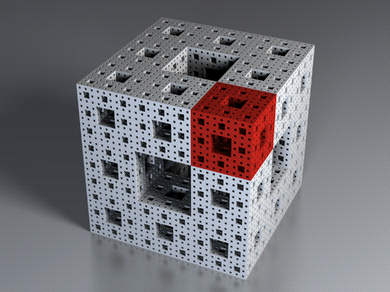
\includegraphics[height=0.4\linewidth]{img/manual/media/menger_sponge.png} 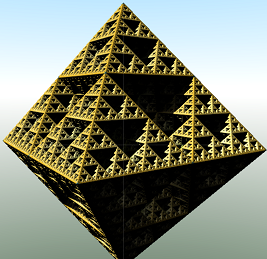
\includegraphics[height=0.4\linewidth]{img/manual/media/sierpinski.png}

\subsection{Mandelbulber Program}\label{mandelbulber-program}

Mandelbulber is an easy to use, handy application designed to help you render 3D
Mandelbrot fractals called Mandelbulb and some other kind of 3D fractals like
Mandelbox, Bulbbox, Juliabulb, Menger Sponge, \ldots{}. The following sections
cover the program interface and give useful information about how to use it.
